% AI-assisted drafting and evidence checking; see the shared AI statement.
\section{三引擎时间预测与分层预警响应}\label{q3:sec}

\subsection{预测对象、信息集与评价设计}\label{q3:sec:design}
针对源区启动时间及下游预警需求，建立机械首次过阈、变形零点外推和动态风险三个互补引擎。
本地对象是源区首次机械启动；外部位移资料的标签是终末或主体失稳；传播响应以给定整体释放为起点。
本地日历时刻 $t$ 统一用UTC，外部记录以原资料相对小时 $s$ 计算，不补写未知的UTC偏移。
对发布时刻 $t_0$ 或 $s_0$，B/C的信息集 $\mathcal F_0$ 仅含发布前观测；A以给定历史重建状态为起点，分列假设可得天气、理想对照和严格首发审核。统一报告
$H\in\{24,48,72\}\,\mathrm h$ 内的事件质量、不发生质量及条件时间区间。
若 $\tau$ 为距发布时刻的等待时间，模型内中央区间定义为
\begin{equation}
 p_H=\Prob(0<\tau\le H\given\mathcal F_0),\qquad
 I^{.95}_H=\left[Q_{.025},Q_{.975}\right](\tau\given0<\tau\le H,\mathcal F_0).
 \label{q3:eq:interval}
\end{equation}
区间端点是相对时长，需加各自发布时刻；其名义水平与观测标签的实际覆盖率分别计算。

外部资料由历史岩坡监测集和Brienz公开记录构成\cite{q3-leinauer2023,q3-loewdata2024}，按物理过程合并为13个终末失稳组，另以Stampa的725天真实观测作为一个右删失组\cite{q3-schild2026}；
Brienz两传感器属于同一组。风险模型的确知生存暴露合计\num{56381.84}小时，失稳标签的时间不确定性单独进入似然。
采用外层留组、训练侧选参，并在同一传感器、发布锚点和时域上配对比较；连续小时及传感器数量均不增加独立事件分母。
本文按本地条件计算、外部分组评价与释放后传播组织三层证据，各层采用对应的时间对象与评价资料。

\subsection{三条时间预测路线}\label{q3:sec:models}
\paragraph{A：机械首次过阈与信息上下界。}
沿用第二问的失稳裕度 $M_\theta=F_{S,\theta}-1$，将结构、解析导热、储排水和损伤状态共同暖启动，定义
\begin{equation}
 \tau_\theta(t_0)=\inf\{h>0:M_\theta(t_0+h)\le0\},\qquad
 \inf\varnothing=+\infty .\label{q3:eq:firstpass}
\end{equation}
实际以逐小时首次非正裕度定位跨阈，并在相邻小时间线性插值；完整随访 $H$ 内无跨阈才判定该时域不启动，随访不足归入未知。
256组共同参数、4种机制和2种强度策略组成2048条设计路径。未来边界采用三份18UTC起报的实际GFS产品\cite{q3-noaa-gfs-products}。
75次逐小时发布各设10条输入轨：两种空间摘要各配0/3/6/9小时假设延迟，另设1条理想轨和1条严格首发轨。
严格轨的首次公开可用时间为空时保持未知。由此产生\num{1536000}条参数路径记录，以及
$75\times10\times(8+1)\times3\times3=\num{60750}$组分布；后三项为机制政策及混合、设计先验和时域。

以归一权重 $w_\theta$ 表示给定设计先验，固定原条件历史下的风险集 $\mathcal R$，令
$R=\sum_{\mathcal R}w_\theta$。
其中 $E_H,N_H,U_H$ 分别为域内已知启动、域内已知不启动和结局未知的质量，满足 $E_H+N_H+U_H=R$。
A的 $p_H$ 条件于 $\theta\in\mathcal R$，从而
\begin{equation}
 \frac{E_H}{R}\le p_H\le\frac{E_H+U_H}{R},\qquad R>0 .\label{q3:eq:bounds}
\end{equation}
原已启动质量保持在风险集外；只有 $U_H=0$ 时给出精确概率，并在事件质量为正时求式\eqref{q3:eq:interval}的分位数。
材料域按发布后实际随访的 $L+1$ 个状态离线诊断，要求全部满足 $T\in[-8,-0.5]\,{}^\circ\mathrm C$及有效正应力$100$--$400\,\mathrm{kPa}$，包含跨阈后状态\cite{q2-mamot2018}；
原未来跨阈支撑集中于p0149-S，其有效正应力为$820.31\,\mathrm{kPa}$，相应结局质量归入 $U_H$。
三时域各\num{20250}组主对照均保留正未知质量；启动下界均为0，上界的总体最小值在24/48小时为0.488584，72小时为0.497717，最大值均为1。
这给出了指定设计的\textbf{信息界}，精确概率与条件分位数记空。
同随访天气对照进一步分解边界替换的作用：在72小时终点，各设计中的最大界面温差为
$2.78954\,{}^\circ\mathrm C$，无量纲裕度差为1.07956；随访内峰值孔压差最大为$40.86915\,\mathrm{kPa}$。
终点状态与过程峰值分别比较，说明天气能够改变水热状态，而当前发布窗的离散跨阈支撑仍由同一结构分支主导。
因此用状态响应评价天气驱动、用信息界评价启动结局，能够保留两种输出各自的分辨能力。

\paragraph{B：逆速度与状态空间外推。}
由发布前最近5点位移回归得到速度绝对值；Weissmiess直接将已给日速度换算为小时速度。取最近16个有限正速度的归一逆速度 $y_i$。
逆速度线性化依据加速失稳的零点关系\cite{q3-fukuzono1985}，本研究分别实现普通最小二乘IV与局部趋势状态空间SS：
\begin{equation}
 \begin{aligned}
 \mathrm{IV}:&\quad y_i=a+b(s_i-s_0)+\varepsilon_i,\qquad\tau=-a/b\ (a>0,b<0),\\
 \mathrm{SS}:&\quad z_i=F(\Delta_i)z_{i-1}+\eta_i,\quad y_i=(1,0)z_i+\epsilon_i,\\[-2pt]
 & F(\Delta)=\begin{pmatrix}1&\Delta\\0&1\end{pmatrix},\quad
 Q(\Delta)=r\rho\begin{pmatrix}\Delta^3/3&\Delta^2/2\\\Delta^2/2&\Delta\end{pmatrix}.
 \end{aligned}\label{q3:eq:deformation}
\end{equation}
SS按实际不等间隔Kalman递推\cite{q3-kalman1960}；$r=\max\{\operatorname{median}_i[(y_i-y_{i-1})^2]/2,10^{-8}\}$，
$\rho=0.01\,\mathrm h^{-3}$。前3点初始化，其余点顺序更新至发布时刻。
IV采用回归系数协方差，SS采用发布时状态协方差，各从联合高斯估计分布中抽取512个样本，条件为当前逆速度为正；
非负趋势对应 $\tau=+\infty$，落入 $(0,H]$ 的比例给出 $p_H$，该时域内的根给出条件区间。
该分布表达当前估计不确定性，SS不另模拟未来过程扰动。历史不足、观测过旧或当前逆速度均值非正时保留弃权。

\paragraph{C：无记录年龄的动态风险。}
令$v_j$为最近6次观测的回归斜率绝对值，$b_j$为最近至多64次观测的相邻速率绝对值中位数，
$c_j$为最近5段之前的6段速率中位数（不足11段时取$b_j$），$\epsilon_j=\max(10^{-6}b_j,10^{-12})$。
构造两个无量纲特征
\begin{equation}
 x_j=\operatorname{clip}_{[-12,12]}\left(
 \log\frac{v_j+\epsilon_j}{b_j+\epsilon_j},\
 \log\frac{v_j+\epsilon_j}{c_j+\epsilon_j}\right).
 \label{q3:eq:features}
\end{equation}
再经训练侧中位数及 $\max(\mathrm{IQR},0.25)$ 缩放并截断为 $z\in[-6,6]^2$。
线性风险与非线性RBF竞争，其中RBF基为
\begin{equation}
 \phi(z)=\left(1,z_1,z_2,
 \{e^{-(z_j-c)^2/2}\}_{j=1,2;\ c=-1,0,1},z_1z_2\right),\quad
 \lambda(s)=e^{\operatorname{clip}(\beta^\top\phi(z(s)),-35,20)}\,\mathrm h^{-1}.
 \label{q3:eq:hazard}
\end{equation}
风险暴露从第6次观测起算，失稳区间内固定标签下界前最后状态。
以暴露起点为累计风险零点，$\Lambda_i(u)=\int_{s_{i,\mathrm{entry}}}^{u}\lambda_i(s)\dif s$，$S_i(u)=e^{-\Lambda_i(u)}$。
失稳区间 $[L_i,U_i]$、精确标签 $T_i$ 和右删失 $C_i$ 的似然贡献分别为
\begin{equation}
 \mathcal L_i=\begin{cases}
 S_i(L_i)-S_i(U_i),&L_i<U_i,\\
 \lambda_i(T_i)S_i(T_i),&L_i=U_i=T_i,\\
 S_i(C_i),&\text{右删失}.
 \end{cases}\label{q3:eq:likelihood}
\end{equation}
分段指数风险以局部常值积分连接暴露与结局\cite{q3-friedman1982}，岭惩罚参数由训练组内留组选取。预测时固定发布前的最后特征，因而
\begin{equation}
 p_H=1-e^{-\lambda_0H},\qquad
 Q_q(\tau\given0<\tau\le H)=-\lambda_0^{-1}\log\!\left[1-q(1-e^{-\lambda_0H})\right].
 \label{q3:eq:hazardquantile}
\end{equation}
主候选为无记录年龄的RBF raw；记录年龄支线只诊断事后选窗的时钟效应。512与1024节点对照保留同一风险集，
原定义锚点上RBF raw的最大概率变化为0.010412，48/72小时Brier变化为0.002959/0.002147。
该对照保持同一物理样本，量化积分网格带来的数值敏感性。

\subsection{分时域结果、覆盖率与提前量}\label{q3:sec:results}
发布锚点按各组随访终点减 $H$ 回顾选取。从14个物理组中，仅在两模型均发布概率且结局已知的相同机会比较，结果见表\ref{q3:tab:brier}；弃权保留为空，72小时Weissmiess无可发布锚点。
24小时的5个可评分组均为阴性，分数主要反映该时域的不报警质量；48/72小时各有4个阳性、4个阴性。
SS在48小时分数较低，RBF raw在72小时较低，支持按监测条件和时域分工。
C全部10个已知结局组的48/72小时分数为0.373917/0.307760；B/C配对比较采用各时域共同组，24小时为5组，48/72小时各为8组。
表中分数按组等权计算为$\mathrm{BS}_H=n_H^{-1}\sum_{i=1}^{n_H}(p_{i,H}-o_{i,H})^2$，
其中$o_{i,H}$仅取确知的0或1；该比较描述所选锚点的有效配对子集。

\begin{table}[htbp]
 \centering\small
 \caption{外部同发布锚点、同有效组的Brier分数（越小越好）}\label{q3:tab:brier}
 \begin{tabular}{ccccc}
 \toprule
 $H/\mathrm h$ & 共同独立组数 & 阳性/阴性 & SS & 无年龄RBF raw\\
 \midrule
 24&5&0/5&0.046924&0.005908\\
 48&8&4/4&0.242887&0.308827\\
 72&8&4/4&0.346922&0.243395\\
 \bottomrule
 \end{tabular}
\end{table}

\begin{figure}[htbp]
 \centering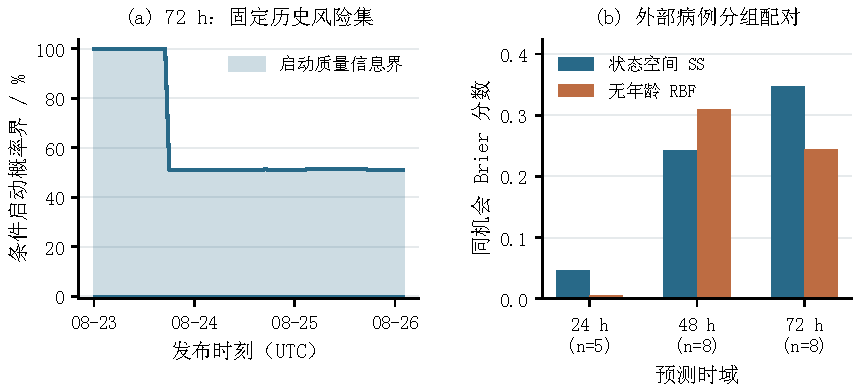
\includegraphics[width=\linewidth]{figures/q3/q3_information_scores.pdf}
 \caption{不同证据层的风险表达。(a)设计等权、机制混合、AOI等权平均及假设零延迟下的72小时信息界，24/48小时在该组合中同形；阴影为条件于原历史风险集的启动概率信息界。(b)表\ref{q3:tab:brier}的外部配对分数，$n$为有效独立组数。两图对象分别为本地条件启动与外部终末失稳。}
 \label{q3:fig:information}
\end{figure}

发布尺度同样影响方法比较。固定共同10个组后，48小时IV/SS的等组Brier在每小时回放为0.17199/0.22659，
在最后48小时原生发布为0.53427/0.49009；72小时分别为0.20396/0.24340及0.45039/0.42196。
两种回放还覆盖不同的观测时期，因此将其解释为发布支持与尺度的联合敏感性，而非单一采样频率效应。

将等待时长转换为源时钟区间 $\widetilde I_i=s_{0,i}+I^{.95}_{H,i}$。对失稳标签 $J_i=[L_i,U_i]$，完整包含为 $J_i\subseteq\widetilde I_i$，相交为 $J_i\cap\widetilde I_i\ne\varnothing$；
完整覆盖、相交覆盖给出区间标签下的保守与宽松统计量。表\ref{q3:tab:coverage}在标签下界前24小时固定发布72小时预测，
每组固定主传感器，无区间者仍留在13个病例机会分母中。

\begin{table}[htbp]
 \centering\small
 \caption{固定截面中央95\%模型区间的外部表现}\label{q3:tab:coverage}
 \begin{tabular}{lccccc}
 \toprule
 模型&有效概率&有限区间&完整包含&相交&点误差中位数/小时\\
 \midrule
 IV&10/13&7/13&3/13&5/13&21.15（7组）\\
 SS&11/13&8/13&6/13&6/13&12.55（8组）\\
 \bottomrule
 \end{tabular}
 \par\smallskip\footnotesize 点误差为预测中位数到标签区间的距离，表列为跨组中位数；括号为有限点分母。
\end{table}
\FloatBarrier

该截面的有限区间平均宽度分别为39.28小时（7组）及44.96小时（8组）；24小时发布提前量来自锚点设计。
另在标签前30天每小时回放，以$p_{72}\ge0.5$产生告警。表\ref{q3:tab:lead}区分首个\textbf{时域内正确告警}与首个任意告警；
前者要求完整标签已落入未来72小时，后者包括远早于该时域的报警。
提前量距标签下界计算，仅在对应有告警组中取中位数；滚动Brienz按两传感器最早告警合并，固定截面使用主传感器。
这种并列报告将及时性与早报分别计量，且总体仍是事先选入的失稳病例。

\begin{table}[htbp]
 \centering\small
 \caption{72小时滚动规则下两种首警统计}\label{q3:tab:lead}
 \begin{tabular}{lcccc}
 \toprule
 模型&时域内正确告警&中位提前量/小时&任意首警&中位提前量/小时\\
 \midrule
 IV&9/13&60.24（9组）&12/13&464.50（12组）\\
 SS&9/13&62.24（9组）&11/13&696.00（11组）\\
 \bottomrule
 \end{tabular}
 \par\smallskip\footnotesize 病例分母为13个失稳组；括号为相应提前量中位数的有效组数。
\end{table}

共同锚点还存在标签上界恰等于时域末端的情形：连续条件分布的97.5\%分位小于 $H$，
使完整包含率为0而相交率可较高。故同锚点评分用于公平概率比较，表\ref{q3:tab:coverage}另列完整标签覆盖。
共形层按独立校准分数的秩 $k=\lceil0.95(m+1)\rceil$检验可达范围\cite{q3-angelopoulos2021}。
实际另留独立校准组为0；即便把外层训练的至多13组作为乐观上界，也有 $k=14>13$。
该计算给出无界的秩可行性结果；本文据此分别呈现模型内条件95\%区间、实际外部覆盖与校准秩。

\subsection{从机械时钟到给定释放后的空间响应}\label{q3:sec:arrival}
以同一base情景连接机械状态和释放物源，最终形成7个运行、4个机械设计、49条目标记录。
模型、法向厚度、密度等20个物理参数逐项保持；紧凑源与全源面、60/120米网格分别记录。
目标到达时钟满足
\begin{equation}
 t_{\mathrm{arr},k}^{(\theta)}=t_{\mathrm{init}}^{(\theta)}+\delta_{\mathrm{rel}}^{(\theta)}+\tau_{\mathrm{prop},k}^{(\theta)}.
 \label{q3:eq:arrival}
\end{equation}
其中机械启动至整体释放的 $\delta_{\mathrm{rel}}$ 保持未知，传播结果按给定整体释放的相对时钟呈现；
图\ref{q3:fig:release}展示的是给定释放后、100米代表点缓冲内格中心厚度达到0.1米的保存帧括号。
p0000和p0072的机械模型未跨阈，仍只作给定释放响应。p0255的全历史跨阈位于7月1日11--12UTC，
后续评价窗则为已不稳左删失，二者分列，不把评价首样本变成窗内新启动。

\begin{figure}[htbp]
 \centering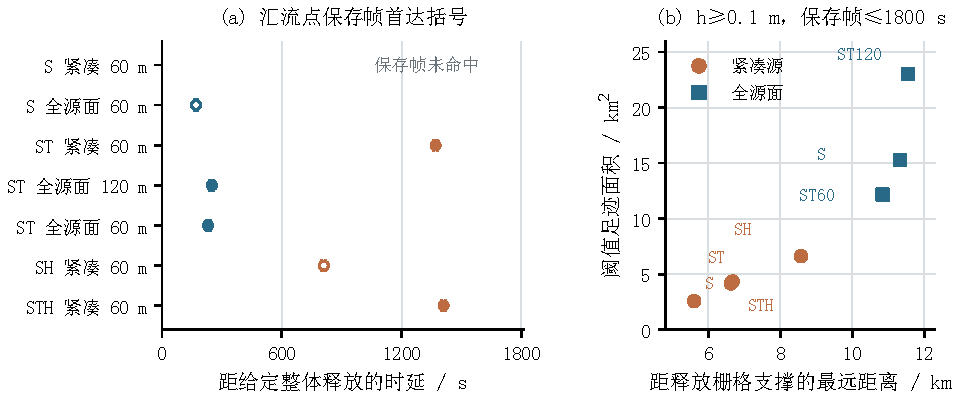
\includegraphics[width=\linewidth]{figures/q3/q3_release_response.pdf}
 \caption{同base情景的条件传播响应。(a)汇流点括号，空心点为仅给定释放、实心点为机械模型已跨阈；“保存帧未命中”保留为观测状态。(b)请求1800秒内、厚度阈值0.1米的足迹面积与距实际正释放栅格足迹的最大格心距离，ST120/ST60为同体积的两个网格。}
 \label{q3:fig:release}
\end{figure}

同体积p0036全源面在120/60米下的足迹为23.0112/12.1608平方千米，支持距离为11.554/10.841千米；
紧凑源对应4.3416平方千米和6.670千米。这些量刻画物源与格网条件下的传播差异，
距离采用释放足迹到受影响格心的欧氏定义，物源边界、原生初态与网格差异共同解释；时间联接按同一情景组合机械状态、阶段转换与传播响应。
由此，本问输出机械状态驱动的信息界、外部可比较的条件时间区间，以及给定释放后的设施响应三类结果，
为气象与变形资料逐步到位时选择相应预警层提供一致接口。
业务更新时，气象引擎先更新水热状态与未知质量；新增变形观测再更新零点与动态风险。
各层同时携带发布时刻、时域和空间对象，使后续观测能够修正相应分布，而不混合不同阶段的时间标签。
\FloatBarrier
\AIcredit
